\documentclass[11pt,a4paper]{report}
\usepackage[textwidth=37em,vmargin=30mm]{geometry}
\usepackage{calc,xunicode,amsmath,amssymb,paralist,enumitem,tabu,booktabs,datetime2,xeCJK,xeCJKfntef,listings}
\usepackage{tocloft,fancyhdr,tcolorbox,xcolor,graphicx,eso-pic,xltxtra,xelatexemoji}

\newcommand{\envyear}[0]{2025}
\newcommand{\envdatestr}[0]{2025-10-30}
\newcommand{\envfinaldir}[0]{webdb/2025/20251030/final}

\usepackage[hidelinks]{hyperref}
\hypersetup{
    colorlinks=false,
    pdfpagemode=FullScreen,
    pdftitle={Web Digest - \envdatestr}
}

\setlength{\cftbeforechapskip}{10pt}
\renewcommand{\cftchapfont}{\rmfamily\bfseries\large\raggedright}
\setlength{\cftbeforesecskip}{2pt}
\renewcommand{\cftsecfont}{\sffamily\small\raggedright}

\setdefaultleftmargin{2em}{2em}{1em}{1em}{1em}{1em}

\usepackage{xeCJK,xeCJKfntef}
\xeCJKsetup{PunctStyle=plain,RubberPunctSkip=false,CJKglue=\strut\hskip 0pt plus 0.1em minus 0.05em,CJKecglue=\strut\hskip 0.22em plus 0.2em}
\XeTeXlinebreaklocale "zh"
\XeTeXlinebreakskip = 0pt


\setmainfont{Brygada 1918}
\setromanfont{Brygada 1918}
\setsansfont{IBM Plex Sans}
\setmonofont{JetBrains Mono NL}
\setCJKmainfont{Noto Serif CJK SC}
\setCJKromanfont{Noto Serif CJK SC}
\setCJKsansfont{Noto Sans CJK SC}
\setCJKmonofont{Noto Sans CJK SC}

\setlength{\parindent}{0pt}
\setlength{\parskip}{8pt}
\linespread{1.15}

\lstset{
	basicstyle=\ttfamily\footnotesize,
	numbersep=5pt,
	backgroundcolor=\color{black!5},
	showspaces=false,
	showstringspaces=false,
	showtabs=false,
	tabsize=2,
	captionpos=b,
	breaklines=true,
	breakatwhitespace=true,
	breakautoindent=true,
	linewidth=\textwidth
}






\newcommand{\coverpic}[2]{
    % argv: itemurl, authorname
    Cover photo by #2~~(\href{#1}{#1})
}
\newcommand{\makeheader}[0]{
    \begin{titlepage}
        % \newgeometry{hmargin=15mm,tmargin=21mm,bmargin=12mm}
        \begin{center}
            
            \rmfamily\scshape
            \fontspec{BaskervilleF}
            \fontspec{Old Standard}
            \fontsize{59pt}{70pt}\selectfont
            WEB\hfill DIGEST
            
            \vfill
            % \vskip 30pt
            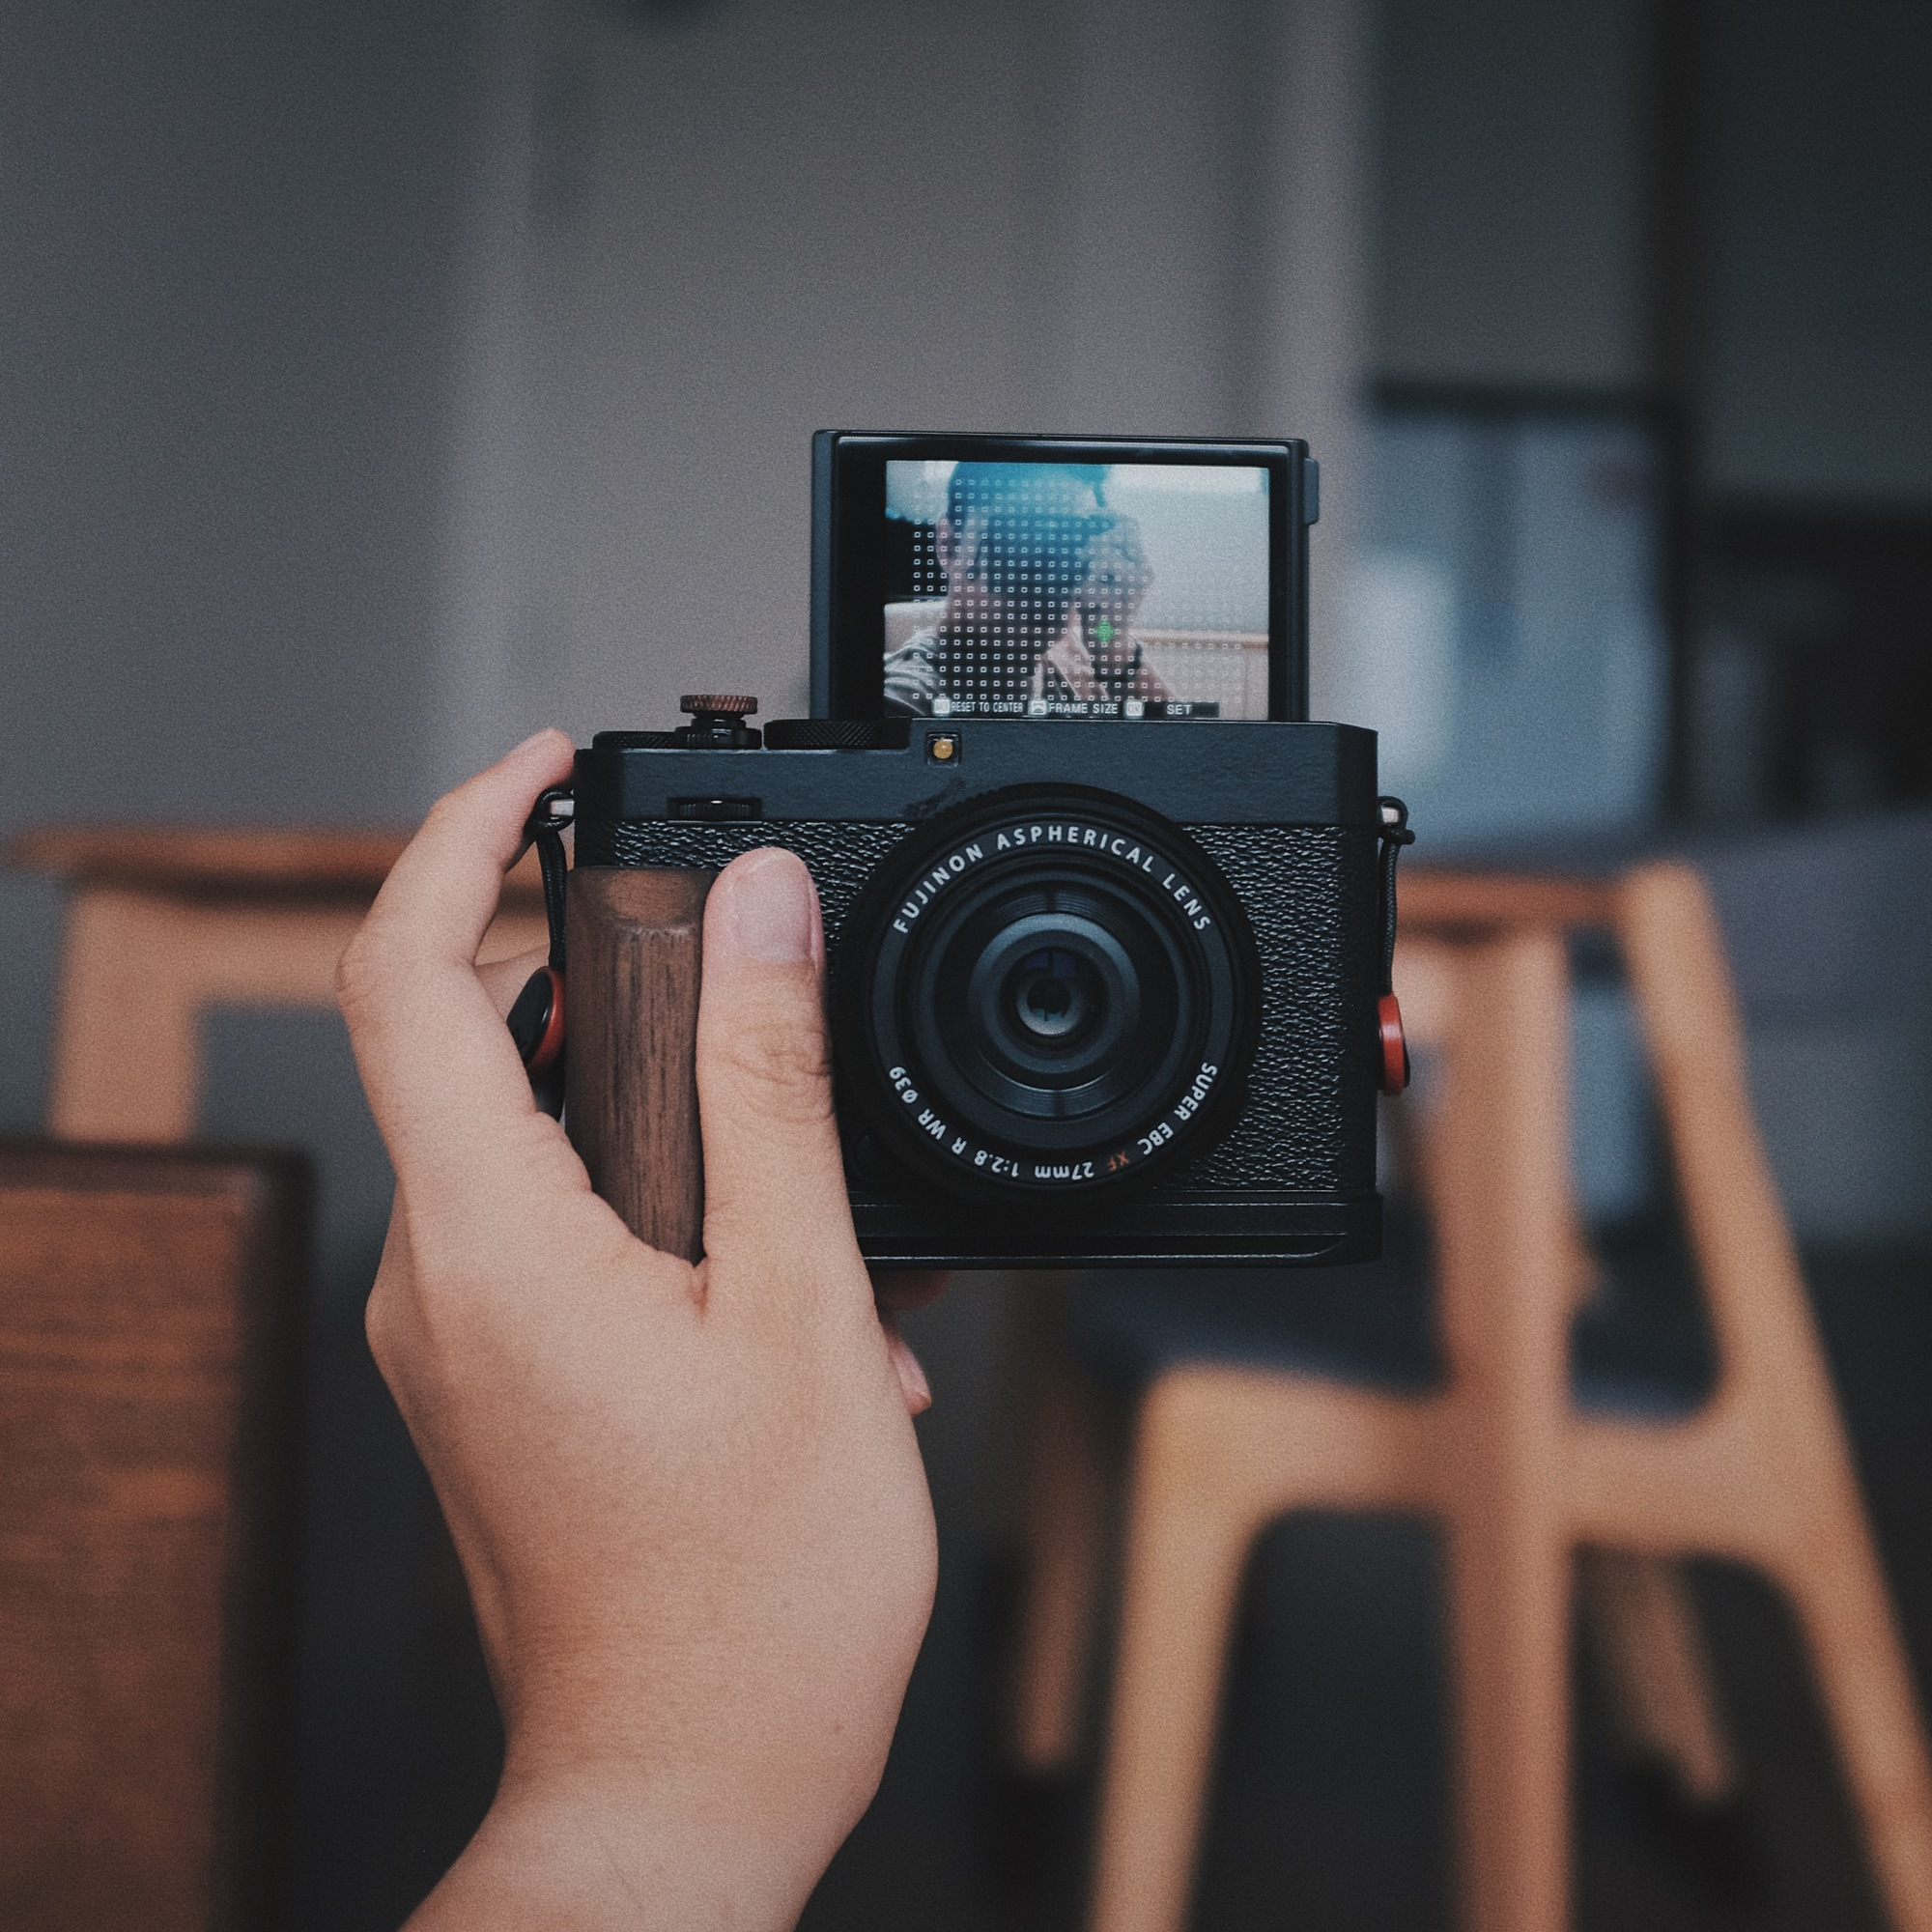
\includegraphics[width=\linewidth]{\envfinaldir/coverpic-prod.jpg}\par
            % \vskip 30pt
            \vfill

            \normalsize\rmfamily\scshape
            \copyright{} The Web Digest Project \hfill\large \envdatestr
        \end{center}
    \end{titlepage}
    % \restoregeometry
}
\newcommand{\simplehref}[1]{%
    \textcolor{blue!80!green}{\href{#1}{#1}}%
}
\renewcommand{\contentsname}{\center\Huge\sffamily\bfseries Contents\par\vskip 20pt}
\newcounter{ipartcounter}
\setcounter{ipartcounter}{0}
\newcommand{\ipart}[1]{
    % \vskip 20pt
    \clearpage
    \stepcounter{ipartcounter}
    \phantomsection
    \addcontentsline{toc}{chapter}{#1}
    % \begin{center}
    %     \Huge
    %     \sffamily\bfseries
    %     #1
    % \end{center}
    % \vskip 20pt plus 7pt
}
\newcounter{ichaptercounter}
\setcounter{ichaptercounter}{0}
\newcommand{\ichapter}[1]{
    % \vskip 20pt
    \clearpage
    \stepcounter{ichaptercounter}
    \phantomsection
    \addcontentsline{toc}{section}{\numberline{\arabic{ichaptercounter}}#1}
    \begin{center}
        \Huge
        \sffamily\bfseries
        #1
    \end{center}
    \vskip 20pt plus 7pt
}
\newcommand{\entrytitlefont}[1]{\subsection*{\raggedright\Large\sffamily\bfseries#1}}
\newcommand{\entryitemGeneric}[2]{
    % argv: title, url
    \parbox{\linewidth}{
        \entrytitlefont{#1}\par\vskip 5pt
        \footnotesize\ttfamily\mdseries
        \simplehref{#2}
    }\vskip 11pt plus 11pt minus 1pt
}
\newcommand{\entryitemGithub}[3]{
    % argv: title, url, desc
    \parbox{\linewidth}{
        \entrytitlefont{#1}\par\vskip 5pt
        \footnotesize\ttfamily\mdseries
        \simplehref{#2}\par\vskip 5pt
        \small\rmfamily\mdseries#3
    }\vskip 11pt plus 11pt minus 1pt
}
\newcommand{\entryitemAp}[3]{
    % argv: title, url, desc
    \parbox{\linewidth}{
        \entrytitlefont{#1}\par\vskip 5pt
        \footnotesize\ttfamily\mdseries
        \simplehref{#2}\par\vskip 5pt
        \small\rmfamily\mdseries#3
    }\vskip 11pt plus 11pt minus 1pt
}
\newcommand{\entryitemHackernews}[3]{
    % argv: title, hnurl, rawurl
    % \parbox{\linewidth}{
    %     \entrytitlefont{#1}\par\vskip 5pt
    %     \footnotesize\ttfamily\mdseries
    %     \simplehref{#3}\par
    %     \textcolor{black!50}{\href{#2}{#2}}
    % }\vskip 11pt plus 11pt minus 1pt
    \begin{minipage}{\linewidth}
            \entrytitlefont{#1}\par\vskip 5pt
            \footnotesize\ttfamily\mdseries
            \simplehref{#3}\par
            \textcolor{black!50}{\href{#2}{#2}}
    \end{minipage}\par\vskip 11pt plus 11pt minus 1pt
}







\begin{document}

\makeheader

\tableofcontents\clearpage




\ipart{Developers}
\ichapter{Hacker News}
\entryitemTwoLinks{Uv is the best thing to happen to the Python ecosystem in a decade}{https://news.ycombinator.com/item?id=45751400}{https://emily.space/posts/251023-uv}

\entryitemTwoLinks{Dithering – Part 1}{https://news.ycombinator.com/item?id=45750954}{https://visualrambling.space/dithering-part-1/}

\entryitemTwoLinks{OpenAI's promise to stay in California helped clear the path for its IPO}{https://news.ycombinator.com/item?id=45750425}{https://www.wsj.com/tech/ai/openais-promise-to-stay-in-california-helped-clear-the-path-for-its-ipo-3af1c31c}

\entryitemTwoLinks{ICE and CBP agents are scanning faces on the street to verify citizenship}{https://news.ycombinator.com/item?id=45749781}{https://www.404media.co/ice-and-cbp-agents-are-scanning-peoples-faces-on-the-street-to-verify-citizenship/}

\entryitemTwoLinks{The Green Tea Garbage Collector}{https://news.ycombinator.com/item?id=45749746}{https://go.dev/blog/greenteagc}

\entryitemTwoLinks{AOL to be sold to Bending Spoons for \$1.5B}{https://news.ycombinator.com/item?id=45749161}{https://www.axios.com/2025/10/29/aol-bending-spoons-deal}

\entryitemTwoLinks{Tailscale Peer Relays}{https://news.ycombinator.com/item?id=45749017}{https://tailscale.com/blog/peer-relays-beta}

\entryitemTwoLinks{Minecraft removing obfuscation in Java Edition}{https://news.ycombinator.com/item?id=45748879}{https://www.minecraft.net/en-us/article/removing-obfuscation-in-java-edition}

\entryitemTwoLinks{Tell HN: Azure Outage}{https://news.ycombinator.com/item?id=45748799}{https://news.ycombinator.com/item?id=45748799}

\entryitemTwoLinks{Composer: Building a fast frontier model with RL}{https://news.ycombinator.com/item?id=45748725}{https://cursor.com/blog/composer}

\entryitemTwoLinks{Tell HN: Azure outage}{https://news.ycombinator.com/item?id=45748661}{https://news.ycombinator.com/item?id=45748661}

\entryitemTwoLinks{Tell HN: Twilio support replies with hallucinated features}{https://news.ycombinator.com/item?id=45748570}{https://news.ycombinator.com/item?id=45748570}

\entryitemTwoLinks{The end of the rip-off economy: consumers use LLMs against information asymmetry}{https://news.ycombinator.com/item?id=45748195}{https://www.economist.com/finance-and-economics/2025/10/27/the-end-of-the-rip-off-economy}

\entryitemTwoLinks{I made a 10¢ MCU Talk}{https://news.ycombinator.com/item?id=45747112}{https://www.atomic14.com/2025/10/29/CH32V003-talking}

\entryitemTwoLinks{Kafka is Fast – I'll use Postgres}{https://news.ycombinator.com/item?id=45747018}{https://topicpartition.io/blog/postgres-pubsub-queue-benchmarks}

\entryitemTwoLinks{Israel demanded Google and Amazon use secret 'wink' to sidestep legal orders}{https://news.ycombinator.com/item?id=45746482}{https://www.theguardian.com/us-news/2025/oct/29/google-amazon-israel-contract-secret-code}

\entryitemTwoLinks{From VS Code to Helix}{https://news.ycombinator.com/item?id=45746478}{https://ergaster.org/posts/2025/10/29-vscode-to-helix/}

\entryitemTwoLinks{Grammarly rebrands to 'Superhuman,' launches a new AI assistant}{https://news.ycombinator.com/item?id=45746401}{https://techcrunch.com/2025/10/29/grammarly-rebrands-to-superhuman-launches-a-new-ai-assistant/}

\entryitemTwoLinks{AWS to bare metal two years later: Answering your questions about leaving AWS}{https://news.ycombinator.com/item?id=45745281}{https://oneuptime.com/blog/post/2025-10-29-aws-to-bare-metal-two-years-later/view}

\entryitemTwoLinks{Aggressive bots ruined my weekend}{https://news.ycombinator.com/item?id=45745072}{https://herman.bearblog.dev/agressive-bots/}\ichapter{Phoronix}
\entryitemGeneric{\hskip 0pt{}AMDGPU With Linux 6.19 Will Support Analog Video Connectors For Old GCN 1.0 GPUs}{https://www.phoronix.com/news/Linux-6.19-AMDGPU-Analog}

\entryitemGeneric{\hskip 0pt{}Mesa 25.2.6 Released With Many Driver Fixes}{https://www.phoronix.com/news/Mesa-25.2.6-Released}

\entryitemGeneric{\hskip 0pt{}Pop!\_OS 24.04 LTS \& COSMIC Desktop Aim For December Stable Release}{https://www.phoronix.com/news/Pop-OS-24.04-In-December}

\entryitemGeneric{\hskip 0pt{}AMD RadeonSI Driver Now Defaults To Enabling ACO For Faster Performance}{https://www.phoronix.com/news/RadeonSI-ACO-Default-Mesa-26.0}

\entryitemGeneric{\hskip 0pt{}AMD Radeon AI PRO R9700 Performance For OpenCL Workloads}{https://www.phoronix.com/review/radeon-ai-pro-r9700-opencl}

\entryitemGeneric{\hskip 0pt{}AMD On Track With openSIL For Zen 6 Platforms, openSIL FAS 1.0 Published}{https://www.phoronix.com/news/AMD-openSIL-October-2025}

\entryitemGeneric{\hskip 0pt{}Intel Compute Runtime 25.40.35563.4 Brings More Panther Lake Changes}{https://www.phoronix.com/news/Intel-CR-25.40.35563.4}

\entryitemGeneric{\hskip 0pt{}AMD XDNA Linux Driver Preps For New Ryzen AI "NPU3A" Revision}{https://www.phoronix.com/news/AMD-Ryzen-AI-XDNA-NPU3A}

\entryitemGeneric{\hskip 0pt{}Apple Plans To Open-Source An LLVM Tool To Security Harden Large C++ Codebases}{https://www.phoronix.com/news/Apple-CPP-Security-Harden-Tool}


\ipart{Developers~~~~(zh-Hans)}
\ichapter{Solidot}
\entryitemGeneric{\hskip 0pt{}Tor Browser 15.0 释出}{https://www.solidot.org/story?sid=82673}

\entryitemGeneric{\hskip 0pt{}Fedora Linux 43 释出}{https://www.solidot.org/story?sid=82672}

\entryitemGeneric{\hskip 0pt{}英伟达成为第一家市值突破 5 万亿美元的公司}{https://www.solidot.org/story?sid=82671}

\entryitemGeneric{\hskip 0pt{}小鼠研究显示头发在 20 天内完全再生}{https://www.solidot.org/story?sid=82670}

\entryitemGeneric{\hskip 0pt{}矮星系发现巨大黑洞}{https://www.solidot.org/story?sid=82669}

\entryitemGeneric{\hskip 0pt{}澳大利亚警方开发大模型解码 Z 世代俚语和表情符号}{https://www.solidot.org/story?sid=82668}

\entryitemGeneric{\hskip 0pt{}外卖正在毁灭美国餐饮业}{https://www.solidot.org/story?sid=82667}

\entryitemGeneric{\hskip 0pt{}侧载究竟意味着什么?}{https://www.solidot.org/story?sid=82666}

\entryitemGeneric{\hskip 0pt{}接近九成 Windows 游戏能在 Linux 上运行}{https://www.solidot.org/story?sid=82665}

\entryitemGeneric{\hskip 0pt{}哈佛本科生六成成绩是 A}{https://www.solidot.org/story?sid=82664}

\entryitemGeneric{\hskip 0pt{}Python 基金会坚持 DEI 放弃美国政府的 150 万美元拨款}{https://www.solidot.org/story?sid=82663}

\entryitemGeneric{\hskip 0pt{}OpenAI 完成公司重组,微软持 27\% 股份和访问技术至 2032 年}{https://www.solidot.org/story?sid=82662}

\entryitemGeneric{\hskip 0pt{}社交圈扩大可能与社会极化相关}{https://www.solidot.org/story?sid=82661}

\entryitemGeneric{\hskip 0pt{}人类迁移的生物量超过所有陆地动物总和 40 倍}{https://www.solidot.org/story?sid=82660}

\entryitemGeneric{\hskip 0pt{}勒索软件的赎金支付比例创新低}{https://www.solidot.org/story?sid=82659}

\entryitemGeneric{\hskip 0pt{}GLP-1 减肥药降低了美国的肥胖率}{https://www.solidot.org/story?sid=82658}

\entryitemGeneric{\hskip 0pt{}阿尔巴尼亚的 AI 部长怀孕了}{https://www.solidot.org/story?sid=82657}

\entryitemGeneric{\hskip 0pt{}OpenAI 和 Anthropic 拥抱不同的商业模式}{https://www.solidot.org/story?sid=82656}

\entryitemGeneric{\hskip 0pt{}小行星撞击地球时恐龙正处于繁盛期}{https://www.solidot.org/story?sid=82655}

\entryitemGeneric{\hskip 0pt{}澳大利亚就微软对 Microsoft 365 订阅费用涨价提起诉讼}{https://www.solidot.org/story?sid=82654}\ichapter{V2EX}
\entryitemGeneric{\hskip 0pt{}[酷工作] 🔥TOP 20 CEX 招聘多个技术研发岗位!}{https://www.v2ex.com/t/1169285}

\entryitemGeneric{\hskip 0pt{}[信息安全] 完蛋,中病毒了,有没有解法?勒索病毒}{https://www.v2ex.com/t/1169284}

\entryitemGeneric{\hskip 0pt{}[iPhone] iPhone 上的``在其他设备上通话''是被 ban 了吗?}{https://www.v2ex.com/t/1169282}

\entryitemGeneric{\hskip 0pt{}[宽带症候群] 有没有用深圳移动的,好像连不上国外 ipv6 了}{https://www.v2ex.com/t/1169281}

\entryitemGeneric{\hskip 0pt{}[输入法] 需要一个尊重上下文的输入法}{https://www.v2ex.com/t/1169280}

\entryitemGeneric{\hskip 0pt{}[程序员] 网页里有办法区分输入法的换行和发送按钮事件吗}{https://www.v2ex.com/t/1169278}

\entryitemGeneric{\hskip 0pt{}[职场话题] 有哪些行业或者企业是不需要 oncall 值班的}{https://www.v2ex.com/t/1169277}

\entryitemGeneric{\hskip 0pt{}[云计算] 微软 Azure 中断}{https://www.v2ex.com/t/1169276}

\entryitemGeneric{\hskip 0pt{}[macOS] safari26 地址栏输入经常卡死}{https://www.v2ex.com/t/1169274}

\entryitemGeneric{\hskip 0pt{}[全球工单系统] 去试用七牛的 AI 推理,现在欠了几百块,账号要没了}{https://www.v2ex.com/t/1169273}

\entryitemGeneric{\hskip 0pt{}[iPhone] 有多少人 Iphone17 系列出现了耳机断联问题}{https://www.v2ex.com/t/1169272}

\entryitemGeneric{\hskip 0pt{}[职场话题] 老员工摸鱼问题}{https://www.v2ex.com/t/1169271}

\entryitemGeneric{\hskip 0pt{}[推广] veo3.1 使用时需要解决的图片问题}{https://www.v2ex.com/t/1169270}

\entryitemGeneric{\hskip 0pt{}[分享创造] [开源][截图]一键表格、公式识别,这款好用的截图软件也太好用了吧}{https://www.v2ex.com/t/1169269}

\entryitemGeneric{\hskip 0pt{}[职场话题] 北京后端开发 怎么找一个不加班或者加班少的外包啊? 比如国企/外企的外包}{https://www.v2ex.com/t/1169268}

\entryitemGeneric{\hskip 0pt{}[问与答] 8TB 文件跨国传输最佳实践是什么?}{https://www.v2ex.com/t/1169267}

\entryitemGeneric{\hskip 0pt{}[分享创造] 写了个 accessLog 解析的小工具}{https://www.v2ex.com/t/1169266}

\entryitemGeneric{\hskip 0pt{}[问与答] 半年没用 Google Voice,俩号全无, tg 也登不上了,天塌了}{https://www.v2ex.com/t/1169264}

\entryitemGeneric{\hskip 0pt{}[推广] ⚡️全新 BaoSIM 平台!卡商直接提供号码, P2P 买卖}{https://www.v2ex.com/t/1169262}

\entryitemGeneric{\hskip 0pt{}[PHP] 记一次微信 access\_token invalid credential, access\_token is invalid or not latest}{https://www.v2ex.com/t/1169261}

\entryitemGeneric{\hskip 0pt{}[宽带症候群] dler 连不上了,官网链接跳转到反诈网站,跑路了?}{https://www.v2ex.com/t/1169260}

\entryitemGeneric{\hskip 0pt{}[Solana] 分享一个 solana 教学 demo 项目, 将您的任意数据永久保存在 solana 主网上 ~}{https://www.v2ex.com/t/1169259}

\entryitemGeneric{\hskip 0pt{}[生活] 隔壁广场舞低频噪音震的头疼,沟通无效,法律难管,求支招!}{https://www.v2ex.com/t/1169258}

\entryitemGeneric{\hskip 0pt{}[iPhone] [黑解] 求教黑解机去可以直接插日本流量卡使用吗?}{https://www.v2ex.com/t/1169257}

\entryitemGeneric{\hskip 0pt{}[互联网] ..}{https://www.v2ex.com/t/1169256}

\entryitemGeneric{\hskip 0pt{}[问与答] 请问,作为一个新人如何学习区块链和所谓的 web3 呢?}{https://www.v2ex.com/t/1169254}

\entryitemGeneric{\hskip 0pt{}[Apple] iPhone17 系列可能存在重大 Bug}{https://www.v2ex.com/t/1169253}

\entryitemGeneric{\hskip 0pt{}[酷工作] [深圳] 影石鸿蒙/KMP 及其他岗位内推}{https://www.v2ex.com/t/1169252}

\entryitemGeneric{\hskip 0pt{}[微信] 微信小程序通知请教}{https://www.v2ex.com/t/1169251}

\entryitemGeneric{\hskip 0pt{}[问与答] 想问下, icloud 拼车有哪些隐私信息会被看到?}{https://www.v2ex.com/t/1169249}

\entryitemGeneric{\hskip 0pt{}[分享创造] M3U8 Player - 免费的在线 M3U8 播放/下载/转换工具}{https://www.v2ex.com/t/1169248}

\entryitemGeneric{\hskip 0pt{}[商业模式] 一人独砍 4k+⭐, BilldDesk 跨平台远程桌面控制!}{https://www.v2ex.com/t/1169247}

\entryitemGeneric{\hskip 0pt{}[酷工作] [北京] AviaGames 内推 |前端/后端/大数据/ 数据 BP/算法/运维/测试/数值策划}{https://www.v2ex.com/t/1169246}

\entryitemGeneric{\hskip 0pt{}[问与答] 这个网站用的是什么知识库程序?}{https://www.v2ex.com/t/1169245}

\entryitemGeneric{\hskip 0pt{}[Android] 安卓手机投屏发现非本路由器的电视}{https://www.v2ex.com/t/1169244}

\entryitemGeneric{\hskip 0pt{}[分享创造] 写了 N 个 AI 应用,我开发了个极简的 LLM 提供商编辑器,每个 AI 应用都用得上,再也不需要为每个 AI 应用重复造轮子了}{https://www.v2ex.com/t/1169243}

\entryitemGeneric{\hskip 0pt{}[远程工作] [远程全职内推] web3 CEX 量化 AI 算法 研发,业务岗都有。薪资 40 万+}{https://www.v2ex.com/t/1169242}

\entryitemGeneric{\hskip 0pt{}[宽带症候群] 上海联通 iptv 出软终端了?小红书看到有位兄弟安装了}{https://www.v2ex.com/t/1169241}

\entryitemGeneric{\hskip 0pt{}[前端开发] rslib 有没有类似 rollup-plugin-serve 的插件。。}{https://www.v2ex.com/t/1169240}

\entryitemGeneric{\hskip 0pt{}[问与答] 谈谈我的消费观}{https://www.v2ex.com/t/1169239}

\entryitemGeneric{\hskip 0pt{}[Windows] Windows 11 LTSC 是否内置 Recall 功能?}{https://www.v2ex.com/t/1169238}

\entryitemGeneric{\hskip 0pt{}[Claude] Claude code 寻 1 车友}{https://www.v2ex.com/t/1169236}

\entryitemGeneric{\hskip 0pt{}[日本語] 有没有什么学习日语的书求推荐。}{https://www.v2ex.com/t/1169235}

\entryitemGeneric{\hskip 0pt{}[分享发现] 纯靠 Ads 投放搞流量,出单了, ROI 打正了,分享一点小经验}{https://www.v2ex.com/t/1169232}

\entryitemGeneric{\hskip 0pt{}[问与答] V2EX 的网页界面,为什么不是宽屏幕界面的,而是那种窄界面,是为了适配手机屏幕么?}{https://www.v2ex.com/t/1169231}

\entryitemGeneric{\hskip 0pt{}[职场话题] ai 改变生活,看不懂代码不会 review 也可以找到开发工作了}{https://www.v2ex.com/t/1169230}

\entryitemGeneric{\hskip 0pt{}[Apple] 真有你的苹果,手机连到 Mac 上变成了充电宝给 Mac 反向充电}{https://www.v2ex.com/t/1169229}

\entryitemGeneric{\hskip 0pt{}[生活] 我结婚快 6 年了,还和前女友有联系,总是忘不了她,怎么办}{https://www.v2ex.com/t/1169228}

\entryitemGeneric{\hskip 0pt{}[创业组队] 有币圈 BD/销售 一起合作搞副业吗?}{https://www.v2ex.com/t/1169227}

\entryitemGeneric{\hskip 0pt{}[问与答] 抓数据遇到滑动验证怎么处理?}{https://www.v2ex.com/t/1169225}


\ipart{Generic News}







\clearpage
\leavevmode\vfill
\footnotesize

Copyright \copyright{} 2023-2025 Neruthes and other contributors.

This document is published with CC BY-NC-ND 4.0 license.

The entries listed in this newsletter may be copyrighted by their respective creators.

This newsletter is generated by the Web Digest project.

The newsletters are also delivered via Telegram channel \CJKunderline{\href{https://t.me/webdigestchannel}{https://t.me/webdigestchannel}}.\\
RSS feed is available at \CJKunderline{\href{https://webdigest.pages.dev/rss.xml}{https://webdigest.pages.dev/rss.xml}}.

This newsletter is available in PDF at
\CJKunderline{\href{https://webdigest.pages.dev/}{https://webdigest.pages.dev/}}.

The source code being used to generate this newsletter is available at\\
\CJKunderline{\href{https://github.com/neruthes/webdigest}{https://github.com/neruthes/webdigest}}.

This newsletter is also available in
\CJKunderline{\href{http://webdigest.pages.dev/readhtml/\envyear/WebDigest-20251030.html}{HTML}} and
\CJKunderline{\href{https://github.com/neruthes/webdigest/blob/master/markdown/\envyear/WebDigest-20251030.md}{Markdown}}.


\coverpic{https://unsplash.com/photos/modern-staircase-with-wooden-accents-and-ambient-lighting-6BSufHdDA4k}{Declan Sun}


\end{document}
